\documentclass{sig-alternate}
%\documentclass{sig-alternate-10pt}
 
\usepackage{verbatim}
\usepackage{graphics}
\usepackage{color}
\usepackage{url}
\usepackage{subfigure}
\usepackage{mdwlist}
\usepackage{floatflt}

\begin{document}

\conferenceinfo{ExtremeCom}{2014}
\CopyrightYear
\crdata

\title{The Breadcrumb Router: Bundle Trajectory Tracking and Geographic Source Routing in DTN
\thanks{\hrule\vspace{0.1in} This work was funded in part by the Laboratory
for Telecommunications Sciences, US Department of Defense.  The opinions
expressed in this paper reflect those of the authors, and do not
necessarily represent those of the Department of Defense or US Federal
Government.}}

\author{
\alignauthor
Tomasz Kalbarczyk\textsuperscript{\#}\quad Brenton
Walker\textsuperscript{*}\quad Christine
Julien\textsuperscript{\#}\quad Angela
Hennessy\textsuperscript{*}\quad\\
Pedro
Santacruz\textsuperscript{\#}\quad Jonas Michel\textsuperscript{\#}\quad Amy
Alford\textsuperscript{\$}\quad \\  
\affaddr{\textsuperscript{\#}The University of Texas at Austin,
Austin, TX}\\
Email: \{tkalbar, pesantacruz, jonasrmichel, c.julien\}@utexas.edu\\
\affaddr{\textsuperscript{*}Laboratory for Telecommunications
Sciences, College Park, MD}\\
Email: brenton@ltsnet.net, ahennes1@math.umd.edu\\
\affaddr{\textsuperscript{\$}The University of Maryland, College Park,
MD}\\
Email: aloomis@math.umd.edu
}


%\numberofauthors{4} 
%\author{
%% 1st. author
%\alignauthor
%Tomasz Kalbarczyk, Pedro Santacruz, Jonas Michel, and Christine Julien\\
%       \affaddr{University of Texas-Austin}\\
%      \email{\{tkalbar, pesantacruz, jonasrmichel, c.julien\}@utexas.edu}
%% 2nd author
%\alignauthor
%Brenton Walker and Angela Hennessy\\
%       \affaddr{Laboratory for Telecommunications Sciences}\\
%       \affaddr{College Park, MD, USA}\\
%       \email{\{brenton, calvin\}@ltsnet.net}
%% 3rd author
%\alignauthor
%Amy Alford\\
%       \affaddr{University of Maryland}\\
%       \affaddr{College Park, MD, USA}\\
%       \email{aloomis@math.umd.edu}
%}

\maketitle

\begin{abstract}
\begin{sloppypar}
Since the dawn of time, man has wanted to know where the heck his bundles went, and to send them back on a specific geo-coded route.  Our new BreadCrumb Router and its associated extension block processors satisfiy this cosmic desire of human existence.  
\end{sloppypar}
\end{abstract}

\category{C.2.1}{Network Architecture and Design}{Store and forward networks}
%\terms{Design, Experimentation, Performance}
\keywords{Delay-Tolerant Networks, Bundle Protocol, Geographic routing}

% -----------------------------------------------
%
%   Introduction
%
% -----------------------------------------------
\section{Introduction}
Since the dawn of time, man has wanted to know where the heck his bundles went, and to send them back on a specific geo-coded route.  Our new BreadCrumb Router and its associated extension block processors satisfiy this cosmic desire of human existence.  

The {\bf traceroute} tool is a staple of traditional IP networks.  It allows a user or administrator to discover the sequence of IP routers their packets pass through between a specific source and destination.  Traceroute works by taking advantage of existing IGMP hop-count and reporting requirements.  Bundle Protocol as defined in RFC5050 has no inherent facility that can achieve this.  Furthermore, because the route a bundle takes may not be stable (one bundle may pass through one sequence of nodes, and a bundle sent a minute later may take another route) it is more salient in a DTN to comprehensively track the entire route of a single bundle, rather than send a series of bundles to probe the network.  Therefore bundle tracking functionality must be built fully as an extension to BP.  Additionally, since in many use cases the geographic mobility of the nodes in a DTN plays an integral part in the routing and delivery of a bundle, tracking the geographic route a bundle follows can be at least as interesting, and possibly {\it more} salient than the logical hops the bundle passes through.

Besides being an illuminating diagnostic tool to understand the behavior of a DTN, tracking the geographic route of a bundle can capture important meta-information related to the contents of a bundle.  The simplest example of this is simply geo-tagging the location where a bundle originated.  A more involved example is tinkerpopping the datums of an oil slick with trajectories with a graph database as described in \cite{jonas-paper} and to be elaborated on here and in the following sections by Jonas and Christine.  Datums: it's the plural of ``datum'' when you're talking about geodetic information, dammit!

Converse to simply geotracking a bundle, we build a prototype router for source geo-routing of a bundle.  In traditional IP networks, extensions to support source routing are defined for both IPv4 and IPv6, but are rarely used and often not supported or blocked.  On the other hand source routing is an integral part of some MANET routing protocols \cite{some-DSR-paper}.  Some reasons source routing could be used are to probe the structure of a newtork, or to specify that packets should avoid sections of a network that are known to be problematic because of congestion, reliability, or security concerns.  Implementing this type of {\it logical} hop-based source routing in DTN is certainly feasible, but in a dynamic mobile network is is difficult to imagine that a source will know exactly which intermediate nodes will be available to ferry its bundles.  Considering the importance of the geographic path in DTN routing, we propose geographic source routing.  In this system a sender can specify both logical (intermediate nodes) and geographic waypoints a bundle must pass through on its way to the destination.

Geographic routing has been proposed and used in many DTN scenarios \cite{paper1,paper2,paper3,paper4,paper5,paper6}.  In most cases greedy geographic routing is used locally to move a bundle closer to a destination.  In other cases large-scale logical hops over an infrastructre network are used to get a bundle to a general geographic area of interest, and then other types of routing take precedence to get the bundle to its final destination.  Source geo-routing is different in that it allows a sender to pre-specify solutions to problems that can arise from greedy geographic routing.  Some of these issues and goals are:
\begin{itemize}
  \item avoiding known dead-ends in the network. I.e. local minima in the greedy geographic routing heuristic.
  \item avoiding geographic areas where unreliability or congestion is anticipated.  For example if a shortest geographic route goes past a baseball stadium, but a game is scheduled for that day, a source may request that a bundle be routed around the expected traffic jam.
  \item ensuring that network coded bundles take sufficiently diverse routes.  Since network coded information can be viewed as a shared secret problem, ensuring that not all of the encodings are ever in the same geographic area could be a security measure in a DTN.
\end{itemize}

\subsection {Prior Work}


% -----------------------------------------------
%
%   Use Cases
%
% -----------------------------------------------
\section{Use Cases}

There are many potential use cases for the GeoTracking and GeoRouting extensions.  For the purposes of testing and demonstration we focus on one in this paper.

% -----------------------------------------------
%   The Maze!
% -----------------------------------------------
\subsection{The Maze!}

The primary use case we investigate in this paper is designed to plausibly and concisely demonstrate the power and functionality of geotracking and source geo-routing in a DTN.

In our scenario a prisoner is held in a maze, and the maze is patrolled by guards who can act as intermediate DTN nodes.  The prisoner sends a bundle, with a GeoTracking block attached, to a rescuer outside the maze.  Initially, when no GeoRouting block is attached, the bundle is routed by the Epidemic routing module.  The GeoTracking block is maintained along the entire route.  Necessarily, then, the first bundle to reach the destination contains enough information to reconstruct the most efficient route through the maze.  The rescuer can remove any backtracked paths the bundle took, and send a bundle with a GeoRouting block attached to the prisoner.

\begin{figure}
\begin{center}
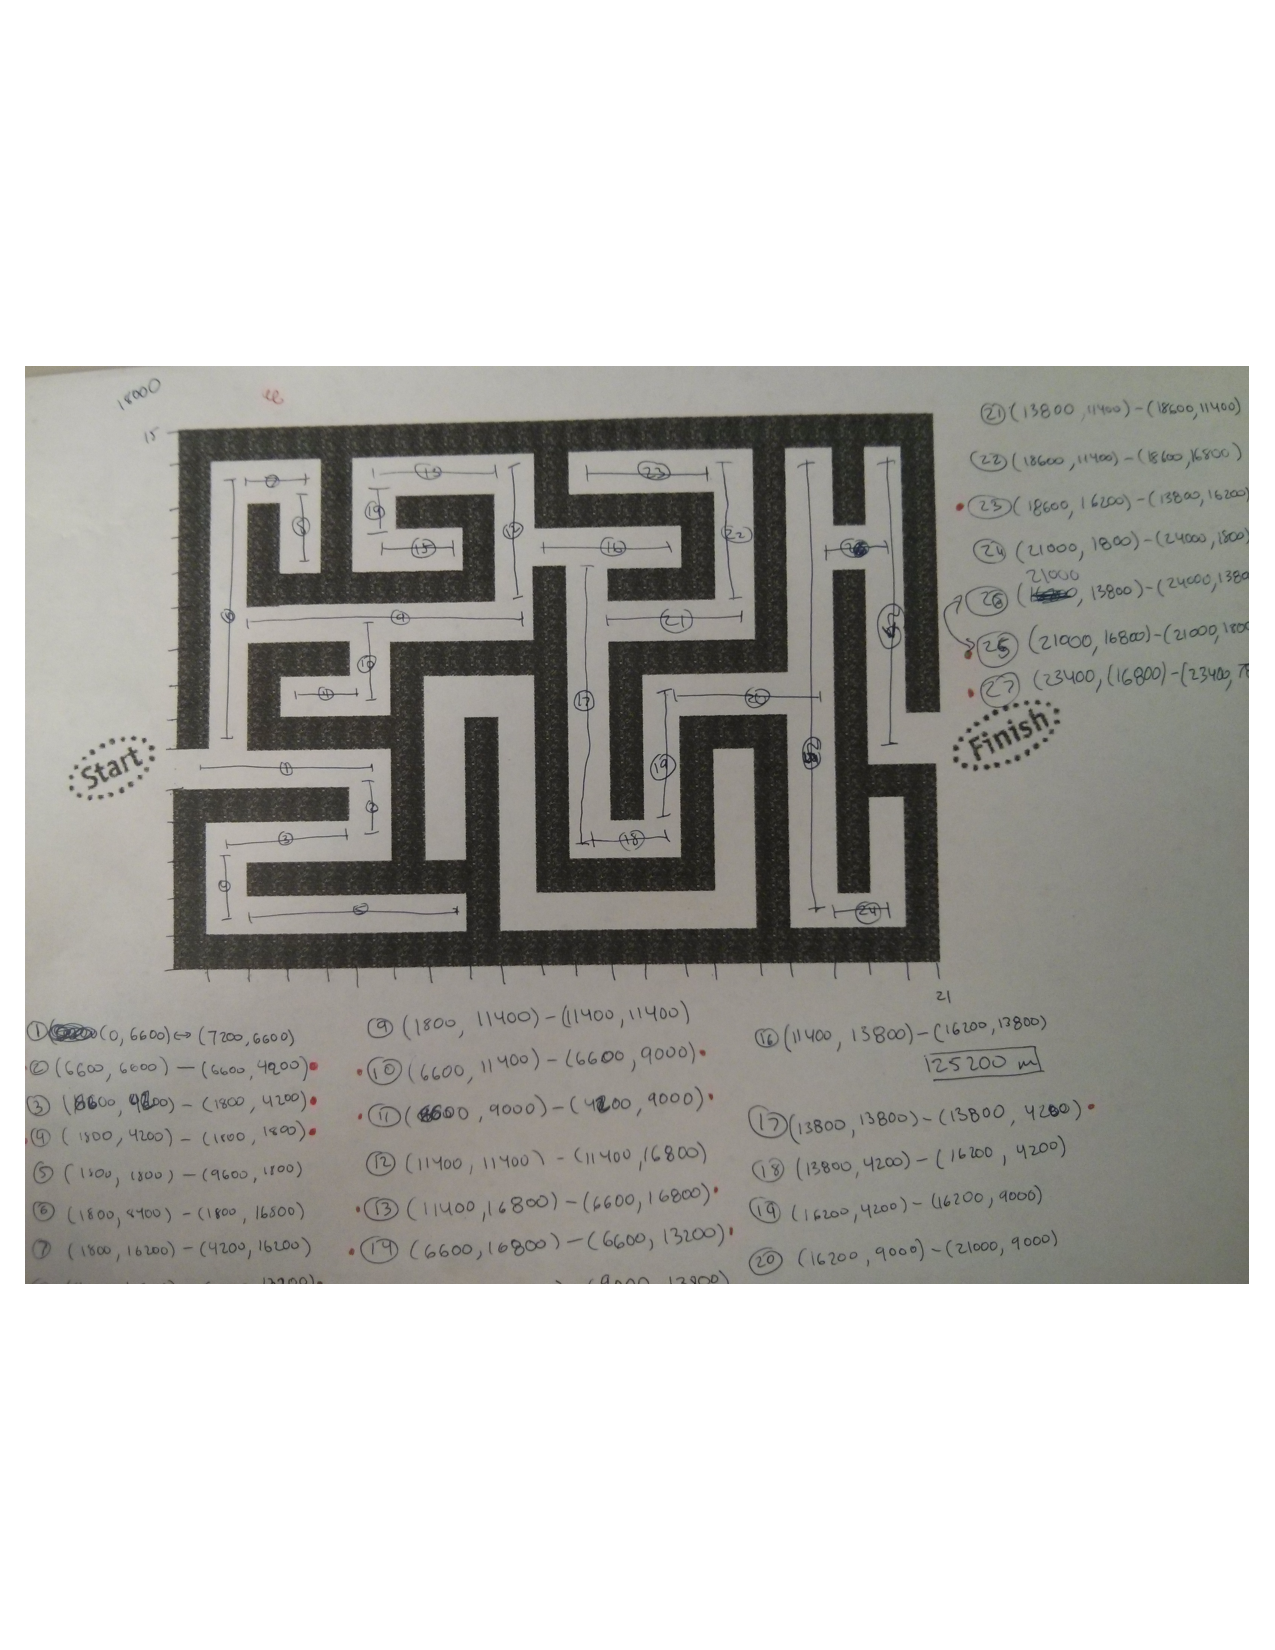
\includegraphics[width=.9\columnwidth]{figures/maze.pdf}
\end{center}
\caption{The maze!}
\label{fig:maze}
\end{figure}

% -----------------------------------------------
%   The Oil Spill!
% -----------------------------------------------
\subsection{The Oil Spill!}


% -----------------------------------------------
%   The Volcano!
% -----------------------------------------------
\subsection{The Volcano!}


% -----------------------------------------------
%   The Sharknado!
% -----------------------------------------------
\subsection{The Sharknado!}




% -----------------------------------------------
%
%   Architecture and Implementation
%
% -----------------------------------------------
\section{Architecture and Implementation}

Here we will describe the design, implementation, and architectural considerations of the GeoTracking and GeoRouting blocks, and the Breadcrumb Router.  All three of these componets involve tying together GPS information that is usually available in a platform-dependent way and is constantly changing, into the BPA.  This is espacially challenging to implement in the IBR-DTN architecture, since all bundle information is held in persistent storage and must be access through bundle filters, and the design ethos dictates that we not create any RAM-based data structures that would grow with the number of bundles held.


% -----------------------------------------------
%   GeoTracking Block
% -----------------------------------------------
\subsection{Geo-tracking Block}

The GeoTracking Block consists of a small header containing parameters for maintaining the block and the number of tracking entries, followed by a series of TrackingEntry fields.  Each TrackingEntry consists of an entry type, and a block of entry data.  The contents of the entry depend on the entry type.

\begin{figure}
\begin{center}
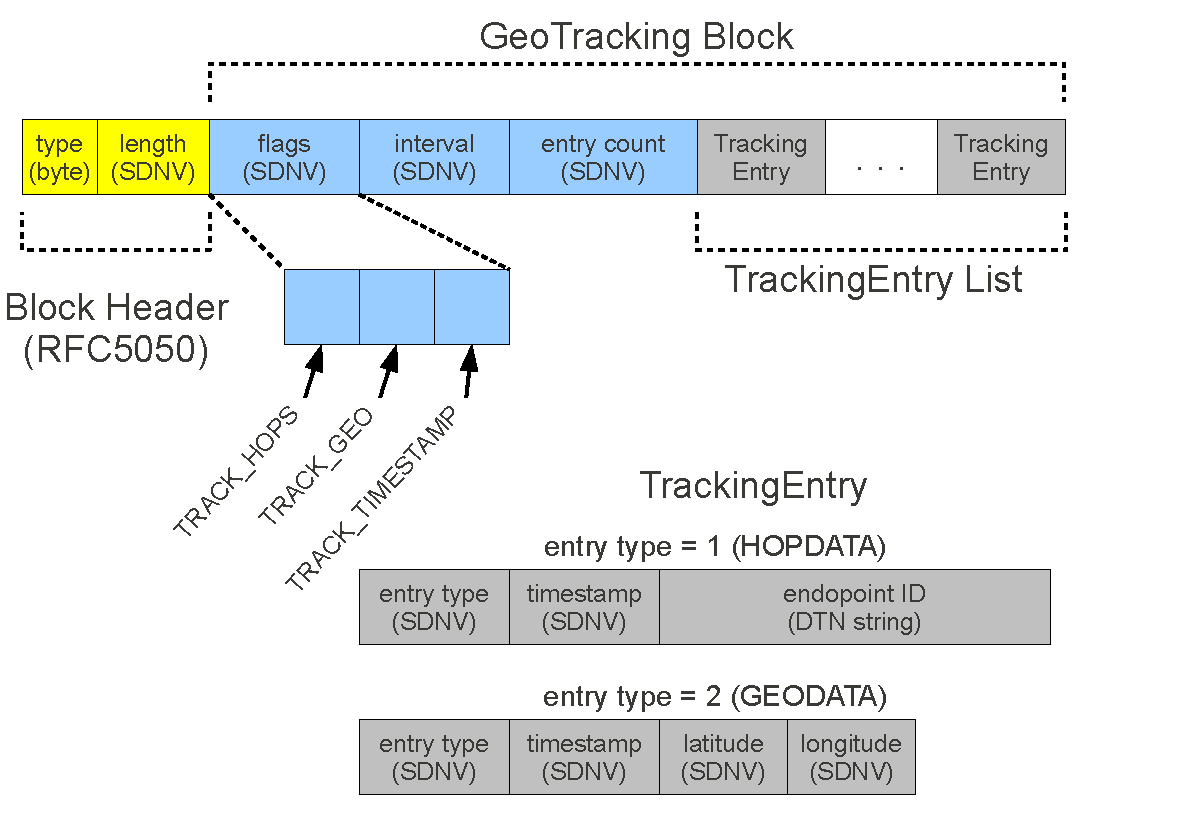
\includegraphics[width=.9\columnwidth]{figures/tracking-block.pdf}
\end{center}
\caption{Format of the GeoTracking Block}
\label{fig:tracking-block}
\end{figure}

The format of the block is depicted in figure~\ref{fig:tracking-block}.  The block header fields apply to every block in a bundle and the format is specified by RFC5050.  In IBR-DTN the block processor only deals with the contents of the block itself, and the BPA strips off the block header.  There are three mandatory fields in the GeoTracking block:
\begin{description}
  \item[Flags] These flags tell intermediate BPAs what information to append to the block.  There are three flags defined: {\bf TRACK\_HOPS} (0x01), {\bf TRACK\_GEO} (0x02), and {\bf TRACK\_TIMESTAMP} (0x04).
  \item[Interval] This tells intermediat BPAs the interval at which to append a GEODATA TrackingEntry to the entry list.  The interval is specified in seconds.
  \item[Entry Count] This is the number of TrackingEntry in the block.
\end{description}

Maintaining and updating the GeoTracking is a dilemma.  We would like for the block stored in the BPA to always be up to date, but it is not feasible to update it in real time for several reasons.  First, the may be many bundles held at the BPA with GeoTracking blocks, and with tracking specified at different intervals.  Updating them all in real time would require quite a few timers, and (in the case of IBR-DTN) reloading/storing each of those bundles from disk each time a new entry is to be attached.  We concluded that it is best to maintain a global GPS log and to only update the GeoTracking block when a bundle is serialized for sending.  The maintainence of this global GPS log then becomes an issue.  In order to completely satisfy the tracking interval requirements of each bundle with a GeoTracking block we would need it to record the node's location at an interval of the GCD of all the tracking intervals.  In our prototype we choose a fixed global interval appropriate to the experiment and bundles can request a {\it less frequent} update.  Finally there is the question of where the GPS log should be maintained.  It could concievably be maintained in the BPA itself, however access to GPS information is a very platform-specific process, whereas a good BPA should be portable.  Also it would require an extra timer or thread in the BPA for a fairly specialized feature.  Our solution is to have a host-specific agent that logs GPS data to a file at an interval chosen by the host.  Each time a GeoTracking block is to be serialized the BPA scans this file for the desired entries and creates the necessary TrackingEntry fields for the Tracking Block.

This method of maintaining GPS data still has some drawbacks, especially in IBRDTN.  First, it requires opening and reading a (potentially long) log file each time a Geotracking block is serialized.  Second, in IBRDTN, because there is no function to "finalize" the contents of a block prior to serializing, the GPS log must be parsed twice.  Once when the block processor calculates the block's length, and again when the actual serialization takes place.  In IBRDTN both the {\bf getLength()} and {\bf serialize()} functions are {\bf const}, so it is not possible to modify any fields of the GeoTracking block itself to cache the state of the block when {\bf getLength()} is called.  This techniclaly creates a race condition between these two calls, where the GPS log may get longer between when {\bf getLength()} and {\bf serialize()} are called.  Resolving these issues completely may require some modifications to the serialization process of IBR-DTN and is reserved for future work (for Johannes).


% -----------------------------------------------
%   GeoRouting Block
% -----------------------------------------------
\subsection{Geo-routing Block}

% -----------------------------------------------
%   The Breadcrumb Router
% -----------------------------------------------
\subsection{The Breadcrumb Router}


% -----------------------------------------------
%
%   Experiments
%
% -----------------------------------------------
\section{Experiments}

\subsection{Mobility Scenario}



% -----------------------------------------------
%
%   Conclusion
%
% -----------------------------------------------
\section{Conclusion}




% Once the sections and outline are solidified, breaking the paper up into separate files will be useful.  For now I'll put the sections inline.
%
%% -----------------------------------------------
%
%   Introduction
%
% -----------------------------------------------
\section{Introduction}
Applications in delay-tolerant networks (DTNs) often desire to both track the path(s) of data through the network and to directly influence the movement of the data. DTNs are almost always integrated into some physical space that also influences that movement of nodes, data, and the phenomena about which the nodes communicate. In traditional IP networks, the {\bf traceroute} tool and {\bf source routing} protocols have assisted in {\em tracking} and {\em directing} packets of data, but the focus has traditionally been on movement through the logical network and not through physical space.

When the physical and logical intertwine, there is a desire for data movement to reflect various aspects of the physical space the data inhabits. We address the dual challenges of {\em tracking} data as it moves through space and time and intentionally {\em routing} data through space and time. As an exemplar of tracking, consider the need for {\em data provenance} in sensing aggregation. As an aggregate collects information sensed about a physical phenomenon, the aggregate may need to dynamically compute the data {\em coverage} by tracking where the aggregate has traveled and collected information~\cite{michel12:spatiotemporal}. As an exemplar of the routing challenge, consider a piece of data that measures the concentration of a gas leak. Users in the area where the gas is expected to dissipate should be warned; this can be accomplished by associating the data item with a route through space and time that captures this expected dissipation. Tracking and routing can also be combined; imagine a generic scenario in which a {\em publisher} generates a piece of data that tracks its movement {\em en route} to a {\em subscriber}. Upon receiving the publication, the subscriber sends a response that must follow the reverse path of the original publication. This generic situation is a stand-in for a variety of concrete applications. For example, the original publication may have reserved some resources along the routing path that the return response relies on. In the later sections of this paper, we use a concrete story behind this more general scenario. Specifically, we consider a maze traversal in which a prisoner in the maze sends a probe that tracks its path as it attempts to exit the maze. When it reaches the exit, the responder (e.g. a rescuer) sends a response packet back to the prisoner along the same path through the maze.

Our problem of tracking differs substantially from the goals of existing utilities, not only in terms of the transition from logical network hops to physical spaces but also because the route a bundle in a DTN takes may not be stable (one bundle may pass through a given sequence of nodes, while a bundle sent just a minute later may take a different route). It therefore may often be important to track the route of {\em each} bundle. In our tracking facility, we track {\em both} logical network hops and the sequence of geographic locations it visits (whether because a device at one location transmits the bundle to a device at a different location or because the device holding the bundle moves). Besides being an illuminating diagnostic tool to understand the behavior of a DTN, tracking a bundle's geographic route can capture important meta-information related to the bundle's contents, as motivated above. 

Source routing, in which a packet carries with it the specific network hops it must traverse, and geographic routing, where packet routing is based on physical locations, have been popular in mobile ad hoc networks~\cite{johnson96:dynamic, karp00:gpsr}. We combine these approaches into a geographically informed version of source routing. Previous approaches to geographic routing predominantly use a {\em greedy} approach in which locally optimal decisions are used to move a bundle incrementally closer to its destination. Our approach to {\em geo-source routing} differs in that it allows the sender to pre-specify a sequence of geo-locations that serve as routing {\em waypoints}. This style of approach can solve a variety of challenges associated with traditional geographic routing. For example by explicitly directing the geographic path of a bundle, our protocol can explicitly route around known dead-ends in the network or around known areas of congestion in the network. Combining this style of geo-routing with other approaches could, for example, ensure that network coded bundles~\cite{petz11:network, widmer05:network} take sufficiently diverse routes through the network.

We introduce the {\sc breadcrumb} router, which implements geo-source routing on DTN bundles that can pre-specify their own delivery paths by providing a combination of geo-locations and logical network hops. 
%In our {\sc breadcrumb} router, elements in this sequence can be {\em required}, meaning that the bundle must touch the specified logical or physical location or {\em optional}, meaning that the sequence serves as a suggestion that the {\sc breadcrumb} router can use simply to guide its decision making. 
Each geo-location comes with a {\em margin of error}, which allows the bundle to get {\em near} the specified location without having to exactly reach it. We also introduce two bundle {\em extension blocks}. The {\em GeoRouting} block holds the sequence of logical and geographical waypoints for geo-source routing. The {\em GeoTracking} block allows any bundle to collect a sequence of locations it visits in both logical and physical space. In our implementation, we rely on a GPS module to provide location information. Throughout the paper, we use the phrases ``GPS location'' or ``GPS coordinates'' to refer to this information, but we note that the GPS framework is a stand-in for any available, potentially highly fine-grained location service framework.  We describe our the {\sc breadcrumb} router and the two extension blocks conceptually and show how we have implemented them in the IBR-DTN implementation of the bundle routing protocol~\cite{IBR-DTN-WASA}. We connect the {\sc breadcrumb} router to our existing Java-based implementation of {\em spatiotemporal trajectories}~\cite{michel12:spatiotemporal}, in which applications can perform expressive computations over data items given knowledge of their movements in space and time and geo-tracking and geo-routing of bundles on a pair of mobility scenarios.



%{\color{blue}
%Since the dawn of time, man has wanted to know where the heck his bundles went, and to send them back on a specific geo-coded route.  Our new BreadCrumb Router and its associated extension block processors satisfy this cosmic desire of human existence.  

%The {\bf traceroute} tool is a staple of traditional IP networks.  It allows a user or administrator to discover the sequence of IP routers their packets pass through between a specific source and destination.  Traceroute works by taking advantage of existing IGMP hop-count and reporting requirements.  Bundle Protocol as defined in RFC5050 has no inherent facility that can achieve this.  Furthermore, because the route a bundle takes may not be stable (one bundle may pass through one sequence of nodes, and a bundle sent a minute later may take another route) it is more salient in a DTN to comprehensively track the entire route of a single bundle, rather than send a series of bundles to probe the network.  Therefore bundle tracking functionality must be built fully as an extension to BP.  Additionally, since in many use cases the geographic mobility of the nodes in a DTN plays an integral part in the routing and delivery of a bundle, tracking the geographic route a bundle follows can be at least as interesting, and possibly {\it more} salient than the logical hops the bundle passes through.

%Besides being an illuminating diagnostic tool to understand the behavior of a DTN, tracking the geographic route of a bundle can capture important meta-information related to the contents of a bundle.  The simplest example of this is simply geo-tagging the location where a bundle originated.  A more involved example is tinkerpopping the datums of an oil slick with trajectories with a graph database as described in \cite{jonas-paper} and to be elaborated on here and in the following sections by Jonas and Christine.  Datums: it's the plural of ``datum'' when you're talking about geodetic information, dammit!

%Converse to simply geotracking a bundle, we build a prototype router for source geo-routing of a bundle.  In traditional IP networks, extensions to support source routing are defined for both IPv4 and IPv6, but are rarely used and often not supported or blocked.  On the other hand source routing is an integral part of some MANET routing protocols \cite{some-DSR-paper}.  Some reasons source routing could be used are to probe the structure of a network, or to specify that packets should avoid sections of a network that are known to be problematic because of congestion, reliability, or security concerns.  Implementing this type of {\it logical} hop-based source routing in DTN is certainly feasible, but in a dynamic mobile network is is difficult to imagine that a source will know exactly which intermediate nodes will be available to ferry its bundles.  Considering the importance of the geographic path in DTN routing, we propose geographic source routing.  In this system a sender can specify both logical (intermediate nodes) and geographic waypoints a bundle must pass through on its way to the destination.

%Geographic routing has been proposed and used in many DTN scenarios \cite{paper1,paper2,paper3,paper4,paper5,paper6}.  In most cases greedy geographic routing is used locally to move a bundle closer to a destination.  In other cases large-scale logical hops over an infrastructure network are used to get a bundle to a general geographic area of interest, and then other types of routing take precedence to get the bundle to its final destination.  Source geo-routing is different in that it allows a sender to pre-specify solutions to problems that can arise from greedy geographic routing.  Some of these issues and goals are:
%\begin{itemize}
%  \item avoiding known dead-ends in the network. I.e. local minima in the greedy geographic routing heuristic.
%  \item avoiding geographic areas where unreliability or congestion is anticipated.  For example if a shortest geographic route goes past a baseball stadium, but a game is scheduled for that day, a source may request that a bundle be routed around the expected traffic jam.
%  \item ensuring that network coded bundles take sufficiently diverse routes.  Since network coded information can be viewed as a shared secret problem, ensuring that not all of the encodings are ever in the same geographic area could be a security measure in a DTN.
%\end{itemize}
%\footnote{Brenton's original text, a lot of which gets reused in the above structure}
%}
%\input{background}
%\input{routing}
%\input{evaluationPharos}
%\input{evaluationNYC}
%\input{evaluationVMT}
%\input{evaluationBrief}
%\input{conclusion}
%\input{related}
% removed in favor of combining related work with "Background" section
%\section*{Acknowledgments}
%This work was funded in part by the US Dept. of Defense. The views expressed are those of the authors and may not necessarily reflect the views of the sponsoring agencies.\\

\bibliographystyle{abbrv}
%\begin{scriptsize}
\bibliography{geobreadcrumb}
%\end{scriptsize}

\end{document}

